\documentclass[11pt,a4paper]{article}

\usepackage[margin=2.5cm]{geometry}
\usepackage{amsmath,amssymb}
\usepackage{bm}
\usepackage{graphicx}
\usepackage{xcolor}
\usepackage[colorlinks=true,linkcolor=blue!60!black,urlcolor=blue!60!black]{hyperref}
\usepackage{cleveref}
\usepackage[section]{placeins}

\title{The Kicked Top from an Island and from the Chaotic Sea\\[0.3em]
  \large Classical map, quantum top and qubit chain at the same initial points}
\author{}
\date{}

\begin{document}
\maketitle

\section{Models and parameters}

All three models are kicked about $x$ and twisted about $z$. The classical map of a unit vector $\bm s=(X,Y,Z)$,
$Z=\cos\theta$, $X+iY=\sin\theta\,e^{i\phi}$, is
\begin{equation}
  \bm s_{n+1} = R_z(kZ')\,R_x(h)\,\bm s_n,\qquad Z'=\big(R_x(h)\bm s_n\big)_z .
\end{equation}
The quantum kicked top of spin $j$ has the Floquet operator
\begin{equation}
  U = e^{-i\epsilon J_z^2}\,e^{-ihJ_x},\qquad \epsilon = \frac{k}{2j}.
\end{equation}
The chain of $n_q=2j$ qubits has the collective spin $\bm J=\frac12\sum_i\bm\sigma_i$ and
\begin{equation}
  U_{\rm chain} = e^{-i\epsilon H_{zz}}\,e^{-ih J_x},\qquad H_{zz}=\sum_{i,l}V_{il}\,\sigma^z_i\sigma^z_l,\quad
  V_{il}=\tfrac14,\qquad hJ_x = \frac h2\sum_i\sigma^x_i ,
\end{equation}
so that $H_{zz}=J_z^2$, $\epsilon = k/n_q$, and $U_{\rm chain}=U$ in the symmetric subspace. Time reversal uses the
backward period $e^{+ihJ_x}e^{-i(2\pi-\epsilon)H_{zz}}$, which inverts $U_{\rm chain}$ up to a global phase.

We take $h=\pi/2$ and $k=2.4$, which divides the classical phase space into regular islands and a chaotic sea of
roughly equal size (\cref{fig:section}). The quantum top has $j=6$ and the chain $n_q=12$ qubits, so
$\epsilon = 2.4/12 = 0.2$ in both. The two initial points are
\begin{itemize}
  \item island: $(\theta_0,\phi_0)=(\pi/2,-\pi/2)$, the centre of the island around $-\hat{\bm y}$ (finite-time
  Lyapunov exponent $\Lambda\approx3\times10^{-4}$ after $1000$ kicks);
  \item chaotic sea: $(\theta_0,\phi_0)=(\pi/2,\pi/4)$ ($\Lambda\approx0.14$).
\end{itemize}
The classical orbit is started at these points, the quantum top and the chain in the spin coherent state
$|\theta_0,\phi_0\rangle$ (for the chain the product state with every qubit along $(\theta_0,\phi_0)$).

\section{Figures}

\begin{figure}[h]
  \centering
  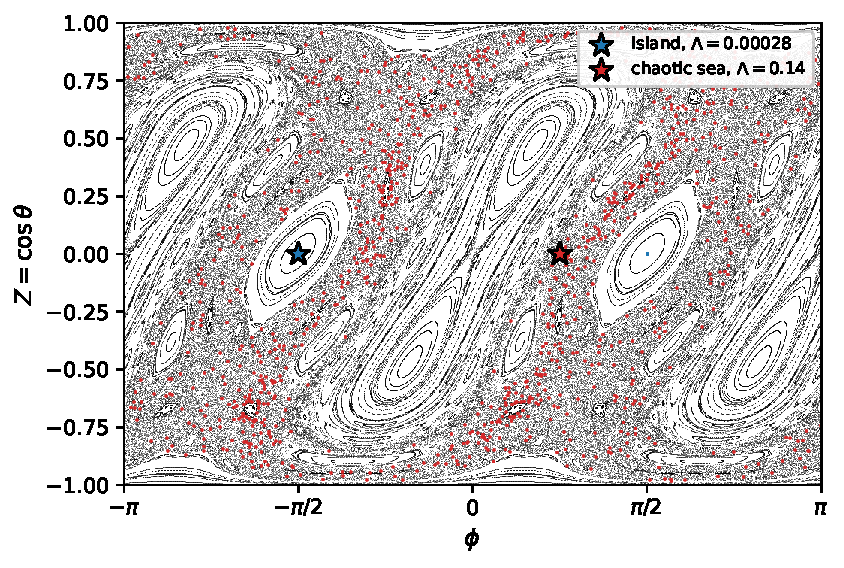
\includegraphics[width=0.75\textwidth]{figures/section.pdf}
  \caption{Classical Poincar\'e section, $h=\pi/2$, $k=2.4$: 1000 kicks of 400 orbits started on a grid (black), and
  the orbits started at the island point (blue) and at the chaotic-sea point (red). Stars: initial points.}
  \label{fig:section}
\end{figure}

\begin{figure}[h]
  \centering
  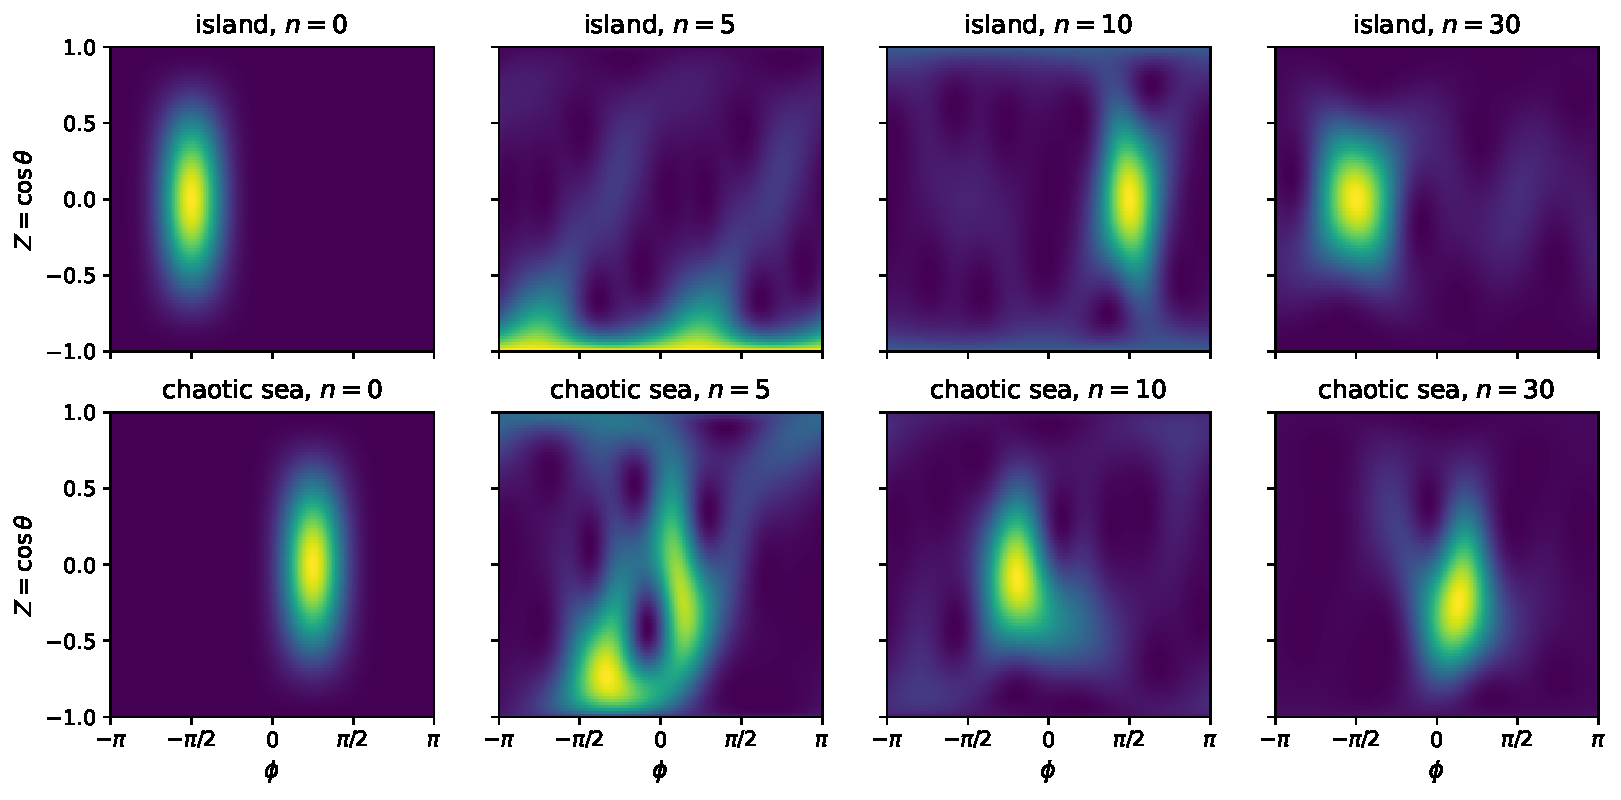
\includegraphics[width=\textwidth]{figures/quantum_husimi.pdf}
  \caption{Husimi distribution of the quantum kicked top, $j=6$, $\epsilon=0.2$, $h=\pi/2$, after $n$ kicks, for the
  coherent state started in the island (top) and in the chaotic sea (bottom). At $j=6$ the coherent state is about as
  large as the island, and the island state tunnels to the symmetric island around $+\hat{\bm y}$ and back.}
  \label{fig:quantum-husimi}
\end{figure}

\begin{figure}[h]
  \centering
  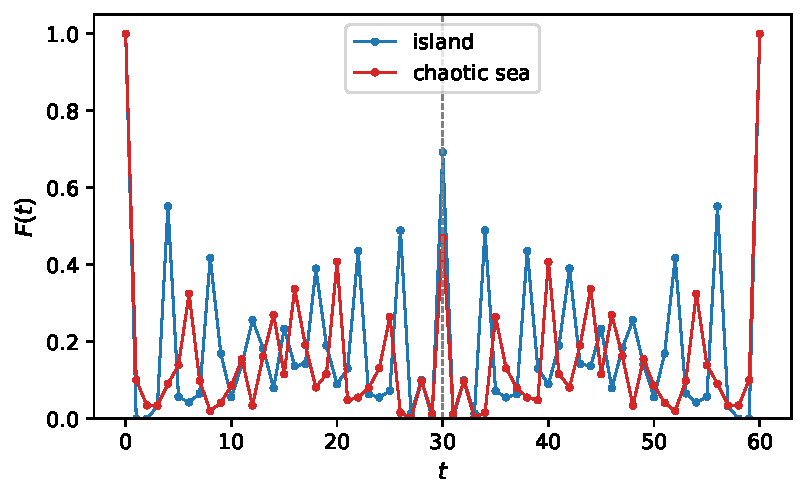
\includegraphics[width=0.75\textwidth]{figures/chain_fidelity.pdf}
  \caption{Fidelity $F(t)=|\langle\psi_0|\psi(t)\rangle|^2$ of the qubit chain, $n_q=12$, $\epsilon=0.2$,
  $h=\pi/2$: $t_r=30$ forward periods, then $t_r$ backward periods. $F(2t_r)-1$ is $8\times10^{-15}$ (island) and
  $-3\times10^{-15}$ (chaotic sea).}
  \label{fig:chain-fidelity}
\end{figure}

\begin{figure}[h]
  \centering
  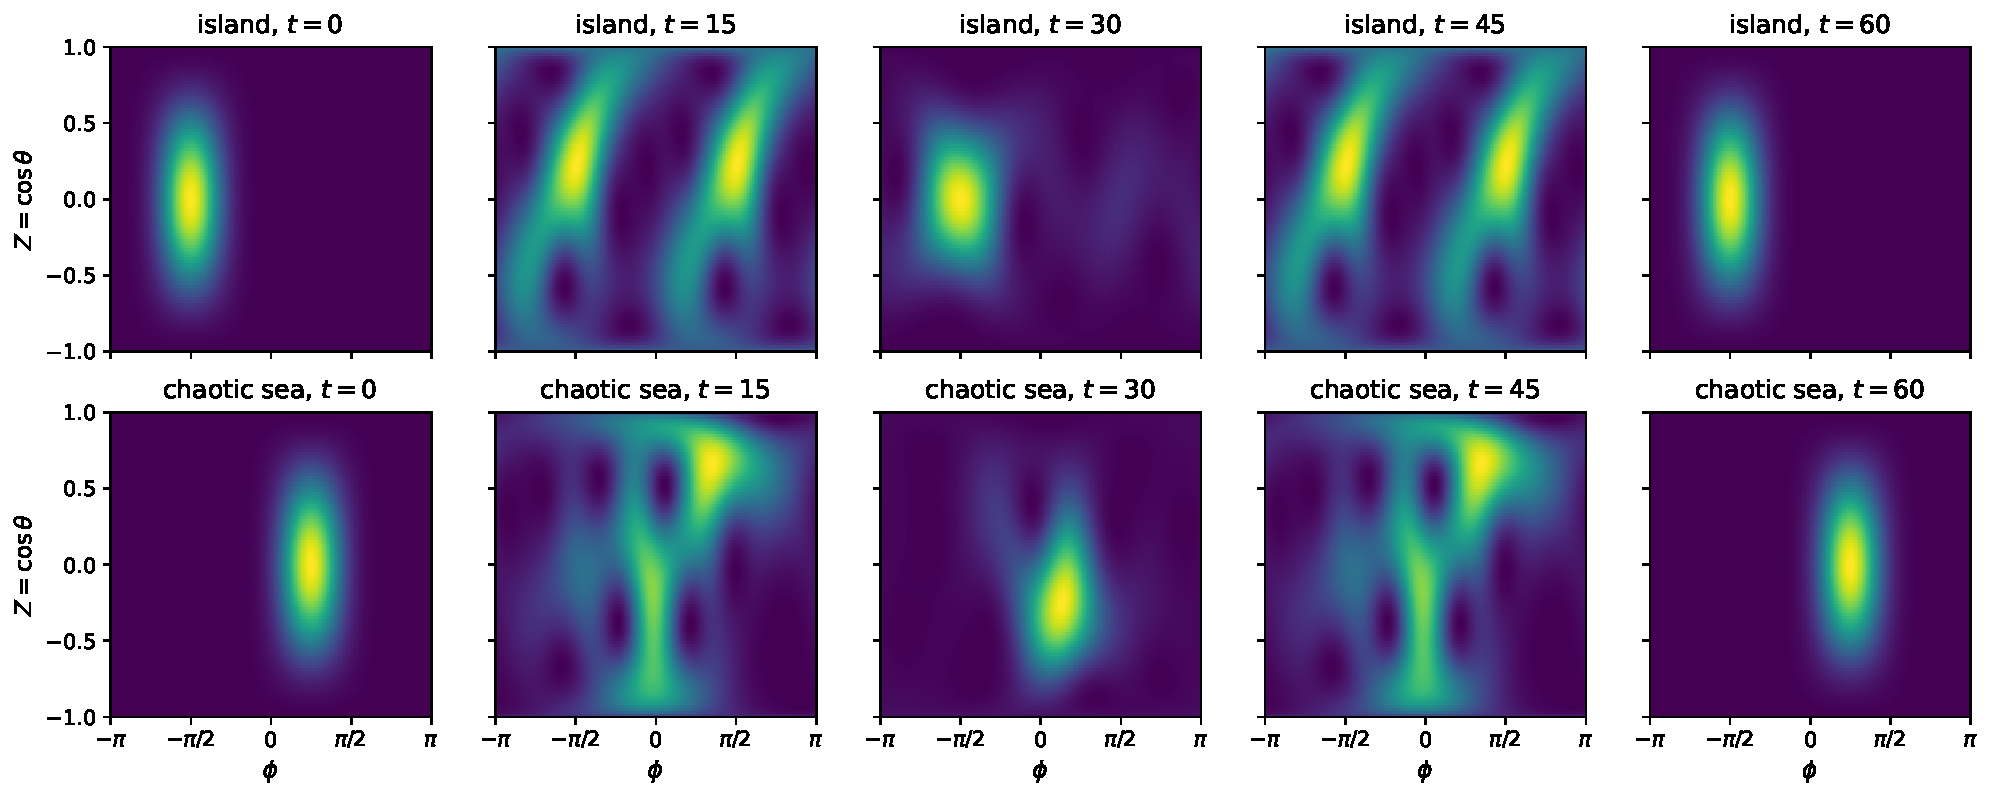
\includegraphics[width=\textwidth]{figures/chain_husimi.pdf}
  \caption{Husimi distribution of the collective spin $\bm J=\frac12\sum_i\bm\sigma_i$ of the chain in the symmetric
  subspace, $n_q=12$, at $t=0$, $t_r/2$, $t_r$, $3t_r/2$ and $2t_r$, for the island (top) and chaotic-sea (bottom)
  initial states. At $t=t_r$ it agrees with the quantum top of \cref{fig:quantum-husimi} at $n=30$ to $10^{-13}$.}
  \label{fig:chain-husimi}
\end{figure}

\end{document}
